\documentclass{article}

\usepackage{commath}
\usepackage{graphicx}
\usepackage{fullpage}
\usepackage{subcaption}
\usepackage{units}
\usepackage{hyperref}
\usepackage{siunitx}
\usepackage{listings}
\usepackage{multicol}
\usepackage{bm}

\lstset{columns=fullflexible,basicstyle=\ttfamily}

\allowdisplaybreaks

\DeclareMathOperator*{\argmin}{argmin}

\title{Time Stretching of the GeV Emission of GRBs: Fermi LAT data vs geometrical model}
\author{
	Maxim S. Piskunov$^{1}$\thanks{\href{mailto:maxit@ms2.inr.ac.ru}{maxit@ms2.inr.ac.ru}} and
	Grigory I. Rubtsov$^{1}$\thanks{\href{mailto:grisha@ms2.inr.ac.ru}{grisha@ms2.inr.ac.ru}} \\
	$^{1}$Institute for Nuclear Research RAS, 117312, Moscow, Russia\\
}

\begin{document}
\maketitle

\begin{abstract}
	Numerous observations confirm that the high energy $(> \unit[100]{MeV})$ emission of gamma ray bursts is delayed with respect to the low energy emission.
	However, the difference of light curves in various high energy bands has not been studied properly.

	In this paper we consider all the bursts observed by Fermi-LAT since 2008 August 4 to 2011 August 1, for which at least $10$ events with energies $\unit[1]{GeV}$ or higher were observed.
	There are $4$ of them: 080916C, 090510, 090902B, and 090926A.
	We study their light curves in two bands, $(\unit[100]{MeV}, \unit[1]{GeV})$ and $(\unit[1]{GeV}, \unit[300]{GeV})$.

	The Kolmogorov-Smirnov test is used to check whether the light curves for these two bands are the same.
	No significant difference was found for 080916C and 090510.
	However, we observed with statistical significance of $3.3 \sigma$, that the higher energy light curve of 090926A is stretched with respect to the lower-energy one, and with statistical significance of $2.2 \sigma$, that the lower energy light curve of 090902B is stretched with respect to the higher-energy one.

	We suggest a simple geometrical model to explain this result.
	The main assumption is the jet opening angle dependence on radiation energy -- the most energetic photons are emitted near the axis of the jet.
	We also assume that all bursts are the same in their rest frames (that is their light curves differ only because of different redshifts and different view directions).
	To test this model, we compute the total energy of the burst, and confirm that it is below the constraint.
	We also compute the fraction of observable bursts in $(\unit[100]{MeV}, \unit[1]{GeV})$ band, which can also be observed in higher energies.
	This fraction matches the observations.
	We predict the distribution of observable stretching factors, which may be tested in the future when more observational data become available.
	Finally, we propose a way to estimate observer's off-axis angles (view directions) based on stretching factors and fractions of high energy photons.
\end{abstract}

\section{Introduction}

	Gamma Ray Bursts (GRBs) are among the most energetic events in the Universe, therefore they might provide new knowledge for particle physics.
	Modern observatories, specifically Fermi \cite{Ackermann:2012kna} and Swift \cite{Gehrels:2004gu} made possible to study these explosions extensively \cite{Vianello:2013ela,Gehrels:2013xd}.
	These and previous studies led to several interesting results.
	For example, the total energy emitted in gamma-rays during a burst was found to be similar among different bursts within an order of magnitude \cite{Bloom:2003wy}.
	This suggests that most of the bursts must have similar energetics in their rest frames.
	Temporal variations of spectra were also studied. The spectral lags were found between different low energy bands \cite{Yi:2005ht}.
	The very high energy radiation was discovered to be extended relative to x-ray emission \cite{Castignani:2014gaa,Lange:2013uh,Vianello:2013ela}.
	We decided to elaborate on that result, and, using the data from Large Area Telescope (LAT) of Fermi, explore the spectral variations between different high energy bands, specifically $(\unit[100]{MeV}, \unit[1]{GeV})$ and $(\unit[1]{GeV}, \unit[300]{GeV})$ (we call them low and high energy bands throughout the paper).
	In particular, we use the Kolmogorov-Smirnov test to compute the time stretching of radiation in one of these bands compared to the other.

	We take the GRB list from the Fermi-LAT catalog \cite{Ackermann:2013zfa}.
	Tables 2 and 4 in \cite{Ackermann:2013zfa} provide the time, durations and locations of the bursts, which we use to download observational data from the LAT Data Server\footnote{\url{http://fermi.gsfc.nasa.gov/cgi-bin/ssc/LAT/LATDataQuery.cgi}}.
	We also download events during a day before the burst, and use the technique introduced in \cite{Rubtsov:2011qq} to estimate background radiation in both energy bands.

	Most of the bursts in the catalog, however, do not have enough events with over $\unit[1]{GeV}$ energies to do desired computations, so we choose only those bursts, from which at least $10$ photons were detected in the high energy band.
	It leaves $4$ of them: 080916C \cite{Tajima:2009az}, 090510 \cite{Ackermann:2010us}, 090902B \cite{Abdo:2009pg} and 090926A \cite{Bregeon:2011bu}.

	For these 4 bursts we compute both high and low energy distributions of photon arrival times, and subtract background estimates from them.
	This makes CDFs non-monotonous and, rigorously speaking, we cannot use the 2-sample Kolmogorov-Smirnov test on it.
	However, since the number of photons is much higher than estimated background, this non-monotonicity is negligible, and will not harm KS-test results much.

	Finally, we stretch the high energy CDF by different factors, and compare it to the low energy CDF using the KS-test.
	If we require $2\sigma$-significant probability to exclude a particular stretching factor, then the stretching factor of $1$ (which means no stretching) is allowed for GRBs 080916C and 090510.
	For the other two bursts the stretching factor of 1 is, however, excluded.
	For GRB 090902B it should be smaller than 1, so the low energy light curve is stretched with respect to the high energy one (see fig. \ref{fig:grb090902B}).
	And for GRB 090926A even more significant deviation from the stretching factor of 1 is observed in the opposite direction.
	The high energy light curve of GRB 090926A is stretched with respect to the low energy one by a factor of at least 1.99 (see fig. \ref{fig:grb090926A}).
	All observed stretching factors are summarized in table \ref{tab:observationResults}.

	We propose that this result can be explained by the curvature effects (that is the effects of the jet geometry).
	These effects were explored by multiple authors \cite{Nakamura:2001kd,Shen:2005ea,Shenoy:2013cba}.
	However, these studies were only concerned with x-ray radiation, and, even more importantly, they assumed that the distribution of radiation sources is homogeneous throughout the jet.
	We propose a contrary idea: that the highest energy radiators are concentrated near the axis of the jet, so that the jet opening angle depends on energy.
	We cannot prove this assumption rigorously, but we have arguments supporting it.

	First of all, there are around 750 GRBs detected by GBM, half of which were in the LAT field of view at the moment of observation \cite{Vianello:2013ela}.
	However, only about 30 of them were detected by the LAT, and only 3 of them were bright in the high energy band.
	If we extrapolate the uniform jet model to very high energies, this observation would mean that these groups of bursts are internally different: some of them produce VHE radiation, while others do not.
	These differences are hard to explain given that burst energetics are similar \cite{Bloom:2003wy}.
	Nevertheless, these differences in burst counts can easily be explained by our model.
	In our model, the opening angle of a jet is inversely proportional to the energy of photons it radiates.
	Therefore the most common scenario is that the off-axis angle of an observer is smaller than the low energy jet opening angle, but much larger than the opening angle of a high energy jet.
	Because of that, most of the bursts can only be seen at low energies.
	The 4 bursts we study in this paper were seen, according to our model, from the lowest off-axis angles.

	Second, consider the plasma right after its ejection from the central engine.
	Two processes happen there simultaneously:
	\begin{enumerate}
		\item{Particles near the jet boundary collide and change their movement directions, therefore increasing the opening angle of the jet.}
		\item{Particles lose energy, therefore decreasing radiation frequency emitted by the jet.}
	\end{enumerate}
	We argue that these two processes are correlated, for they happen due to the same particle interaction processes.
	And since they are correlated, jets with larger opening angles should have lower energies, which is the assumption we are trying to justify.

	\begin{figure}
        \centering
        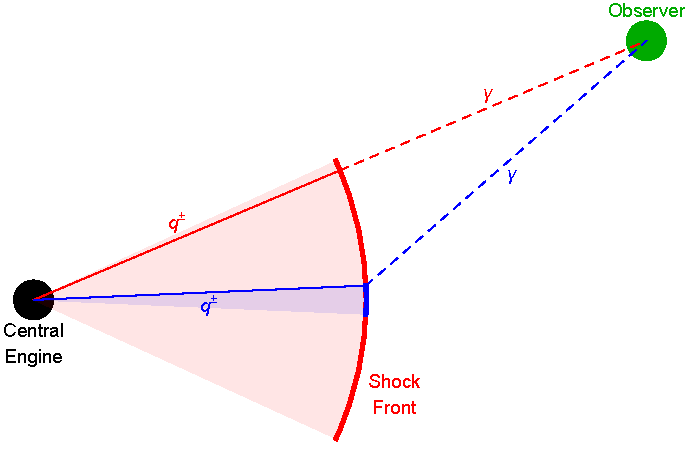
\includegraphics[width=0.7\textwidth]{modelOverview}
        \caption{
        	Model Overview.
        	Here red and blue cones represent the regions through which low and high energy plasma propagates.
        	In case depicted the observer's off-axis angle is smaller than the opening angle of the low energy jet, so, due to the relativistic beaming effect, the most of the observable low energy photons will travel along the straight line from the central engine.
        	Also, the observer's off-axis angle is larger that the opening angle of the high energy jet, so the high energy radiation will still originate near the center of the jet (because it is the only place where there are high energy radiators).
        	The observation time of a photon is a sum of two things: the time interval spent in plasma as a radiator (which approximately equals to the distance from the central engine to the point of emission); and the time interval from emission to detection (which is the distance from the point of emission to the observer's location).
        	Given a position of the shock front, this sum is larger for high energy photons.
        	Because of that, high energy emission will be observed later throughout the burst duration, therefore the high energy light curve will be stretched.
        }
        \label{fig:modelOverview}
	\end{figure}

	\begin{figure}
		\centering
		\hspace*{\fill}
		\begin{subfigure}{0.45\textwidth}
			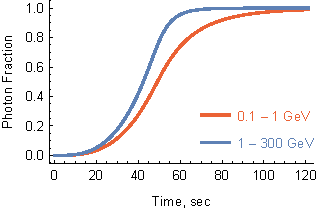
\includegraphics[width=\textwidth]{sampleLightCurveLogNegative}
			\label{fig:sampleLightCurveLogNegative}
			\caption{Stretching factor $\kappa = 0.821$, redshift $z = 1.82$, off-axis angle $\chi = 0$.}
		\end{subfigure}
		\hfill
		\begin{subfigure}{0.45\textwidth}
			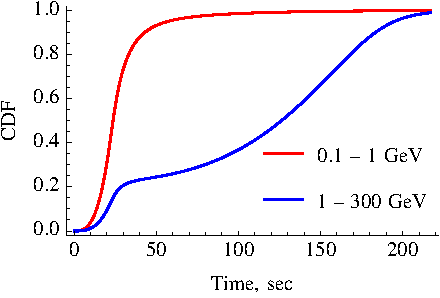
\includegraphics[width=\textwidth]{sampleLightCurveLogPositive}
			\label{fig:sampleLightCurveLogPosivie}
			\caption{Stretching factor $\kappa = 2.26$, redshift $z = 2.106$, off-axis angle $\chi = 5.41 \times 10^{-3}$.}
		\end{subfigure}
		\hspace*{\fill}
		\caption{
			High and low energy light curves produced by the geometrical model.
			Burst parameter values are the same as discussed in section \ref{sec:parameters}.
		}
		\label{fig:sampleLightCurves}
	\end{figure}

	Finally, our assumption is able to explain the non-trivial stretching factor of both GRBs 090902B and 090926A.
	Detailed computations will be described in the following sections, but you can see the main idea on figure \ref{fig:modelOverview}.
	The computations confirm that this qualitative picture is indeed correct.
	You can see a sample light curves on figure \ref{fig:sampleLightCurves}, and predicted distribution of stretching factors on figure \ref{fig:kappaDistribution}.

\section{Observations}
\label{sec:observations}

\subsection{Burst Data Download}

\begin{table}
	\centering
	\small
	\begin{tabular}{ l | S[table-format=9.3] | S[table-format=3.3] | S[table-format=-2.3] | S[table-format=1.5] | S[table-format=2.1] | S[table-format=3.1] }
		\multicolumn{1}{ c |}{GRB} & $\mathrm{GBM\ Trigger\ Time}$ & $\mathrm{R.A.}$ & $\mathrm{Dec.}$ & $\mathrm{Location\ Error}$ & $T_{05}$ & $T_{95}$ \\
		\multicolumn{1}{ c |}{Name}& $\mathrm{MET,\ sec}$ & $\mathrm{J2000,\ deg}$ & $\mathrm{J2000,\ deg}$ & $\mathrm{deg}$ & $\mathrm{sec}$ & $\mathrm{sec}$ \\
		\multicolumn{1}{ c |}{\texttt{name}} & $\mathrm{\texttt{time}}$ & \texttt{location.ra} & \texttt{location.dec} & \texttt{location.err} & \texttt{startOffset} & \texttt{endOffset} \\
		\hline
		080825C	&	241366429.105	&	233.9  	&	 -4.5  	&	0.75   	&	 3.2	&	 29.4	\\
		080916C	&	243216766.614	&	119.85 	&	-56.64 	&	0.0001 	&	 5.0	&	209.8	\\
		081006 	&	244996175.173	&	136.32 	&	-62.05 	&	0.52   	&	 0.7	&	115.0	\\
		081024B	&	246576161.864	&	322.95 	&	 21.2  	&	0.22   	&	 0.1	&	191.0	\\
		090217 	&	256539404.560	&	204.83 	&	 -8.42 	&	0.35   	&	 6.2	&	 68.0	\\
		090323 	&	259459364.630	&	190.71 	&	 17.053	&	0.0001 	&	15.9	&	293.9	\\
		090328 	&	259925808.510	&	 90.67 	&	-41.715	&	0.0002 	&	18.8	&	652.9	\\
		090510 	&	263607781.971	&	333.55 	&	-26.583	&	0.0004 	&	 0.6	&	 45.6	\\
		090626 	&	267683530.880	&	170.03 	&	-33.49 	&	0.22   	&	52.2	&	299.9	\\
		090902B	&	273582310.313	&	264.94 	&	 27.324	&	0.001  	&	 7.7	&	825.0	\\
		090926A	&	275631628.990	&	353.4  	&	-66.32 	&	0.01   	&	 5.5	&	225.0	\\
		091003 	&	276237347.585	&	251.52 	&	 36.625	&	0.0005 	&	 3.9	&	452.6	\\
		091031 	&	278683230.850	&	 71.49 	&	-57.65 	&	0.23   	&	 3.1	&	206.2	\\
		100116A	&	285370262.240	&	305.01 	&	 14.43 	&	0.17   	&	 3.0	&	141.0	\\
		100414A	&	292904423.990	&	192.11 	&	  8.693	&	0.0005 	&	17.4	&	288.6	\\
		110120A	&	317231981.230	&	 61.5  	&	-12.0  	&	0.36   	&	 0.5	&	112.8	\\
		110428A	&	325675112.410	&	  5.59 	&	 64.849	&	0.00001	&	10.7	&	407.6	\\
		110721A	&	332916465.760	&	333.2  	&	-38.5  	&	0.20   	&	 0.1	&	239.0	\\
		110731A	&	333803371.954	&	280.504	&	-28.537	&	0.0001 	&	 3.0	&	 24.1
	\end{tabular}
	\caption{Burst data used in our study. The third row contains the corresponding \texttt{GRBurst} class variable names. The data is taken from the tables 2 and 4 of \cite{Ackermann:2013zfa}. \url{https://github.com/maxitg/GammaRays/blob/master/GRObservations/bursts}}
	\label{tab:bursts}
\end{table}

Before we start to compute the Kolmogorov-Smirnov probabilities, we need to download the actual observational data from the Fermi LAT data server.
We take the data about the bursts from the catalog \cite{Ackermann:2013zfa}, which contains all the bright bursts seen by the LAT since 2008 August 4 to 2011 August 1.
Specifically, we take 4 pieces of information from the tables 2 and 4 there:
\begin{itemize}
	\item{
		GBM trigger time (table 2).
		It is used as a reference point for the GRB time.
	}
	\item{
		Location of the GRB (table 2).
		We need burst locations to filter out photons coming from other sources.
	}
	\item{
		Location error (table 2).
		Location errors are used to improve accuracy of filtering, specifically to avoid losing statistics by filtering too much.
	}
	\item{
		$T_{05}$ -- $T_{95}$ interval of the LAT-detected emission (table 4).
		We need precise intervals for two things.
		First, to understand where is the fixed point of the stretching ($T_{05}$ is used as a proxy for that).
		Second, the burst interval is used to download events data from the data server.
	}
\end{itemize}
The data obtained is summarized in table \ref{tab:bursts}.

Finally, to download the data about observed photons, we fill the form at the LAT data server front page with the following values:
\begin{itemize}
	\item{
		{\bf Object name or coordinates}.
		Here the coordinates are filled from the table \ref{tab:bursts}.
	}
	\item{
		{\bf Coordinate system}.
		J2000.
	}
	\item{
		{\bf Search radius (degrees)}.
		$60$.
		Events will be filtered by location later by using the point spread functions (PSFs) of the LAT.
	}
	\item{
		{\bf Observation dates}.
		To have a decent safety margin, we extend the duration of the burst by $50\%$ to both past and future relative to the table \ref{tab:bursts} time ranges.
		So, we fill in the following values:
		\begin{align*}
			\texttt{time} + \texttt{startOffset} &- 0.5\left(\texttt{endOffset}-\texttt{startOffset}\right),\\
			\texttt{time} + \texttt{endOffset} &+ 0.5\left(\texttt{endOffset}-\texttt{startOffset}\right)
		\end{align*}
	}
	\item{
		{\bf Time system}.
		MET.
	}
	\item{
		{\bf Energy range (MeV)}.
		$100,\,300000$.
		This includes our both energy ranges.
	}
	\item{
		{\bf LAT data type}.
		Extended.
	}
	\item{
		{\bf Spacecraft data}.
		Checked.
		It is required for both events filtering, and calculation of the PSFs and exposure maps.
	}
\end{itemize}

For background estimation, we also download observational data during a day before the burst.
All the values are put the same into the form, except for the time range:
\begin{align*}
	\texttt{time} + \texttt{startOffset} &- 0.5\left(\texttt{endOffset} - \texttt{startOffset}\right) - 86400,\\
	\texttt{time} + \texttt{startOffset} &- 0.5\left(\texttt{endOffset} - \texttt{startOffset}\right)
\end{align*}

Before reading the data, we need to apply the basic filtering as described in Fermi guidelines.
Two tools from the Fermi Science Tools package are used for that task (the same filtering is applied to both burst and background data).

The first one is \texttt{gtselect}\footnote{\url{http://fermi.gsfc.nasa.gov/ssc/data/analysis/scitools/help/gtselect.txt}}.
It filters the Earth limb emission.
We run the tool with the following parameters\footnote{\url{http://fermi.gsfc.nasa.gov/ssc/data/analysis/scitools/explore_latdata_burst.html}}:
\begin{lstlisting}
gtselect infile=[eventFile] outfile=filtered.fits
	ra=INDEF dec=INDEF rad=180 tmin=INDEF tmax=INDEF emin=100 emax=300000
	zmax=100 evclass=0 convtype=-1 evtable=EVENTS
\end{lstlisting}
Here \texttt{[eventFile]} is the file downloaded in the previous step.

The second one is \texttt{gtmktime}\footnote{\url{http://fermi.gsfc.nasa.gov/ssc/data/analysis/scitools/help/gtmktime.txt}}. It uses the spacecraft file as well as events file, and filters out time periods when Fermi LAT was not operational. Running \texttt{gtmktime} is also required for exposure maps calculation, which we'll need later on. Parameters are the following\footnote{\url{http://fermi.gsfc.nasa.gov/ssc/data/analysis/scitools/data_preparation.html}}:
\begin{lstlisting}
gtmktime scfile=[spacecraft] sctable=SC_DATA
	filter="DATA_QUAL>0 && LAT_CONFIG==1" roicut=yes
	evfile=filtered.fits evtable=EVENTS outfile=timed.fits
	apply_fiter=yes
\end{lstlisting}
where \texttt{[spacecraft]} is the FITS file containing the spacecraft data.

Now, with basic filtering done, we can read events data from \texttt{timed.fits}. This file, however, contains observations of a large area of the sky. Before using the data obtained from it, we should perform a more elaborate filtering by location using the point spread function of Fermi LAT. The procedure is described in the following section.

\subsection{Point Spread Functions and Location Filtering}

\texttt{gtpsf}\footnote{\url{http://fermi.gsfc.nasa.gov/ssc/data/analysis/scitools/help/gtpsf.txt}} tool requires the livetime map to generate the PSFs. This map is computed by \texttt{gtltcube}\footnote{\url{http://fermi.gsfc.nasa.gov/ssc/data/analysis/scitools/help/gtltcube.txt}} with the following parameters:
\begin{lstlisting}
gtltcube evfile=timed.fits evtable=EVENTS scfile=[spacecraft] sctable=SC_DATA
	outfile=ltcube.fits
	dcostheta=0.025 binsz=1 phibins=0 tmin=0 tmax=0 zmax=180 zmin=0
\end{lstlisting}

Having the maps, we can compute the PSFs:
\begin{lstlisting}
gtpsf expcube=ltcube.fits outfile=psf_[IrfName].fits outtable=PSF irfs=[IrfName]
	ra=[RA] dec=[DEC] emin=100 emax=1000000 nenergies=41 thetamax=30 ntheta=300
\end{lstlisting}
Here \texttt{[RA]} and \texttt{[DEC]} are the coordinates of the burst, and \texttt{[IrfName]} is the Instrument Response Function, which depends on photon's event class (transient, source, clean, or ultraclean) and conversion type (back or front). The list of IRF names can be obtained with the \texttt{gtirfs}\footnote{\url{http://fermi.gsfc.nasa.gov/ssc/data/analysis/scitools/help/gtirfs.txt}} tool. We need to compute PSFs for all of them.

To understand how to use obtained PSFs, imagine a stream of photons coming from some source located at some coordinates $\theta, \phi$. Ideally, all the coordinates measured for the photons coming from the source should be the same. However, due to measurement errors, they would be spread across some region of the sky. If we find the region such that, say, $95\%$ of photons coming from the source are measured inside of it, we can filter out all the other photons without losing too much statistics, and significantly reducing background. \texttt{gtpsf} approximates these regions as circles, and the files generated in the previous step contain the observation probability densities as functions of distance from the source and photon energies. We, however, need an integral quantity, that is given the radius, we want to know the fraction of photons observed inside the circle of this radius. We can compute this fraction by summing over the probability densities:
\begin{align*}
	p\left(n\right) &= \int_0^n \texttt{pdf[i]} 2\pi \sin\left(\texttt{angles[i]}\right) \dif i \\
	&\approx \sum_{i=0}^{n} \frac{\texttt{pdf[i]} + \texttt{pdf[i+1]}}{2} 2\pi \left(\cos\left(\texttt{angles[i]}\right) - \cos\left(\texttt{angles[i+1]}\right)\right)
\end{align*}
Here \texttt{pdf[i]} is the probability density in the point separated from the source by an angle \texttt{angles[i]}. And $p\left(n\right)$ is the probability to observe a photon closer to the source than \texttt{angles[n]}. We find probabilities for intermediate angles by linear interpolation. Finally, we can compute the inverse value $\theta_{\text{spread}}\left(p\right)$ (that is a distance as a function of probability) by binary search. Note, that $\theta_{\text{spread}}\left(p\right)$ depends on the photon energy, event class, and conversion type. We should use the appropriate function for each photon. The spread angles for intermediate energies are linearly interpolated.

Finally, to finish the filtering, we filter out all the photons, for which their location is separated from the source by more that $\theta_{\text{spread}}\left(0.95\right) + \texttt{location.err}$, where \texttt{location.err} is the uncertainty in the burst location (see table \ref{tab:bursts}).

Now we have a decent set of photons, which we can use for analysis. However, some of the photons in this set are still originated from background, and not from the source. We cannot filter out these photons, but we can substitute a linear component of background by estimating it from a long time period before the burst. In order to perform this computation, we'll need an exposure map, which will be discussed in the following section.

\subsection{Exposure Maps and Background Estimation}

The exposure map can be computed with the \texttt{gtexpcube2}\footnote{\url{http://fermi.gsfc.nasa.gov/ssc/data/analysis/scitools/help/gtexpcube2.txt}} tool. We use the following parameter set for it:
\begin{lstlisting}
gtexpcube2 infile=ltcube.fits cmap=none outfile=expcube_[IrfName].fits irfs=[IrfName]
	nxpix=360 nypix=180 binsz=1 coordsys=CEL xref=0 yref=0 axisrot=0
	proj=CAR ebinalg=log emin=100 emax=1000000 enumbins=40
	ebinfile=NONE bincalc=EDGE ignorephi=no thmax=180 thmin=0 table=Exposure
\end{lstlisting}
The generated \texttt{expcube} files contain exposures as functions of energy and location on the sky\footnote{Note, that R.A. coordinates in the \texttt{expcube} FITS files are indexed in reverse order and starting from 180. For example, $\texttt{ra[0]}=180$, $\texttt{ra[1]}=179$, and so on.}. We use trilinear interpolation to compute exposures for all energies and locations.

Knowing the exposures, we can now use the method introduced in the appendix of \cite{Rubtsov:2011qq} to estimate the linear component of background from the data observed before the burst. We compute two background estimates: for low and high energy bands. Because the background of transient class photons may depend on the spacecraft position, we have to filter them completely.

\subsection{KS-test}

We take care of remaining background by using the following functions with the Kolmogorov-Smirnov test:
\begin{equation}
	\Phi_i\left(t\right) = \frac{p_i\left(T_1, t\right) - b_i \frac{t-T_1}{T_2-T_1}}{p_i\left(T_1, T_2\right) - b_i}
\end{equation}
Here $\left(T_1, T_2\right)$ is the time range of observations, $p_i\left(t_1, t_2\right)$ is the number of photons observed in the time range $t_1$ to $t_2$ in the $i$'s energy band ($i=\text{low},\text{high}$ are for the low and high energy bands respectfully), and $b_i$ is the estimated number of background photons for the time range $T_1$ to $T_2$ in the $i$'s energy band.

The numbers of degrees of freedom (used as an input for the KS-test) are $p_i\left(T_1, T_2\right) - b_i$.

While we did not prove it, we assume that the Kolmogorov-Smirnov statistics computed for these functions with provided number of degrees of freedom has a similar distribution to that of the KS-statistics for ordinary CDFs (that is CDFs with no background).

Finally, we compute KS-probabilities for pairs $\Phi_\text{low}\left(t\right), \Phi_\text{high}\left(\kappa t\right)$ to obtain the allowed ranges for stretching factors $\kappa$. We evaluate stretching factors in the range $\texttt{STRETCHING\_MIN} = 0.1$ to $\texttt{STRETCHING\_MAX} = 10.$ with a logarithmic step of $\texttt{STRETCHING\_STEP} = 1.001$.

As a result of such calculation we can constrain the range of allowed stretching factors to values for which the KS-probabilities are not too small, in other words, given the sigma-significance value, compute the range outside of which stretching factors are elliminated by observations.

You can see the results of such computation in the following section.

\subsection{Results}

Out of 19 bursts studied, only 4 have at least 10 high energy events remaining after filtering, and thus eligible for the computation of stretching factors. The results of this computation are shown on figures \ref{fig:grb080916C}, \ref{fig:grb090510}, \ref{fig:grb090902B}, \ref{fig:grb090926A} and table \ref{tab:observationResults}.

Out of these 4 bursts, two (080916C and 090510) have stretching factors compatible with $\kappa = 1$ within $2\sigma$ range.

GRB 090926A has, however, high energy radiation stretched with respect to low energy signal (that is $\kappa > 1$). In contrast to that, GRB 090902B has low energy radiation stretched with respect to high energy signal ($\kappa < 1$).

So we obtained a preliminary (for significance is only $2\sigma$) result that the stretching factors for observable bursts might be both larger and smaller than $1$.

\begin{figure}
        \centering
        \begin{subfigure}{0.49\textwidth}
                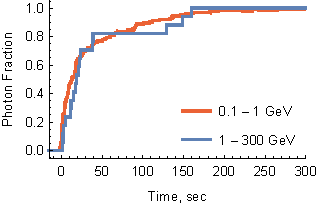
\includegraphics[width=\textwidth]{lightCurve080916C}
                \label{fig:lightCurve080916C}
        \end{subfigure}
        \begin{subfigure}{0.49\textwidth}
                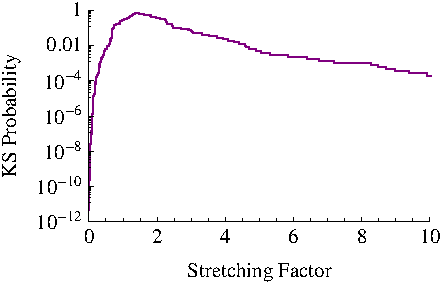
\includegraphics[width=\textwidth]{probabilities080916C}
                \label{fig:probabilities080916C}
        \end{subfigure}
        \caption{GRB 080916C results. Stretching factor is compatible with $\kappa = 1$ within $2\sigma$.}
        \label{fig:grb080916C}
\end{figure}

\begin{figure}
        \centering
        \begin{subfigure}{0.49\textwidth}
                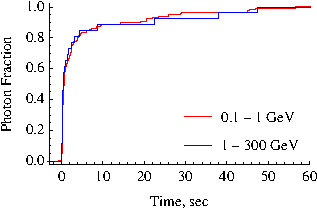
\includegraphics[width=\textwidth]{lightCurve090510}
                \label{fig:lightCurve090510}
        \end{subfigure}
        \begin{subfigure}{0.49\textwidth}
                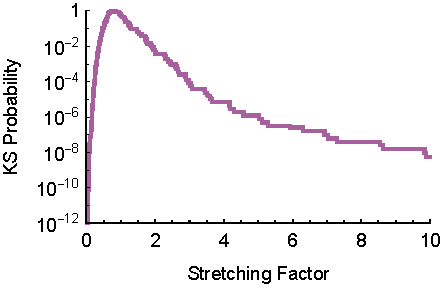
\includegraphics[width=\textwidth]{probabilities090510}
                \label{fig:probabilities090510}
        \end{subfigure}
        \caption{GRB 090510 results. Stretching factor is compatible with $\kappa = 1$ within $1\sigma$.}
        \label{fig:grb090510}
\end{figure}

\begin{figure}
        \centering
        \begin{subfigure}{0.49\textwidth}
                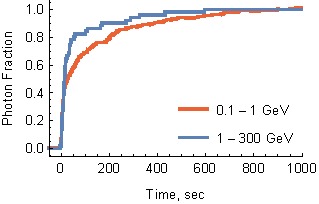
\includegraphics[width=\textwidth]{lightCurve090902B}
                \label{fig:lightCurve090902B}
        \end{subfigure}
        \begin{subfigure}{0.49\textwidth}
                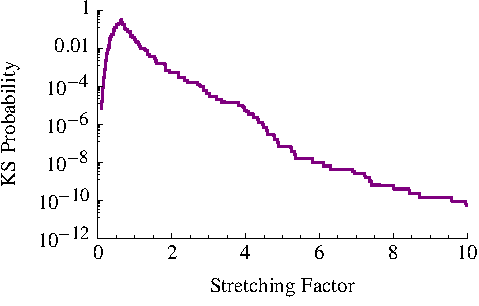
\includegraphics[width=\textwidth]{probabilities090902B}
                \label{fig:probabilities090902B}
        \end{subfigure}
        \caption{GRB 090902B results. Low energy radiation is stretched ($\kappa < 1$) with significance of $2.2\sigma$.}
        \label{fig:grb090902B}
\end{figure}

\begin{figure}
        \centering
        \begin{subfigure}{0.49\textwidth}
                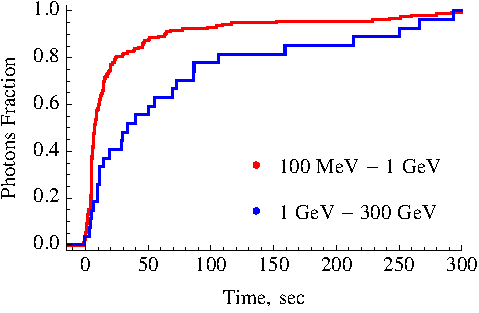
\includegraphics[width=\textwidth]{lightCurve090926A}
                \label{fig:lightCurve090926A}
        \end{subfigure}
        \begin{subfigure}{0.49\textwidth}
                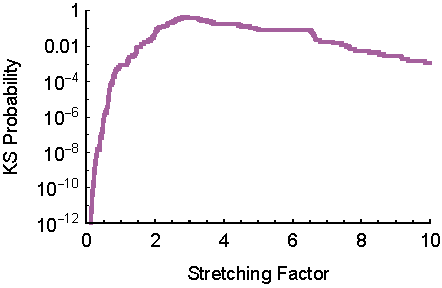
\includegraphics[width=\textwidth]{probabilities090926A}
                \label{fig:probabilities090926A}
        \end{subfigure}
        \caption{GRB 090926A results. High energy radiation is stretched ($\kappa > 1$) with significance of $3.3\sigma$.}
        \label{fig:grb090926A}
\end{figure}

\begin{table}
	\centering
	\small
	\begin{tabular}{ l | S[table-format=2.3]@{\; -- \;}S[table-format=2.3] | S[table-format=2.3]@{\; -- \;}S[table-format=2.3] | S[table-format=2.3]@{\; -- \;}S[table-format=2.3] | S[table-format=2.3]@{\; -- \;}S[table-format=2.3] | S[table-format=2.3]@{\; -- \;}S[table-format=2.3] }
		\multicolumn{1}{ c |}{GRB} & \multicolumn{2}{ c |}{$1\sigma$} & \multicolumn{2}{ c |}{$2\sigma$} & \multicolumn{2}{ c |}{$3\sigma$} & \multicolumn{2}{ c |}{$4\sigma$} & \multicolumn{2}{ c }{$5\sigma$} \\
		\hline
		080916C	&	1.04  & 2.24	&	0.67 & 3.32	&	0.42 & 5.83	&	0.19 & 14.9		&	0.087 & 35.7	\\
		090501	&	0.58  & 1.1		&	0.43 & 1.61	&	0.32 & 2.29	&	0.22 &  3.03	&	0.17  &  5.11	\\
		090902B	&	0.629 & 0.635	&	0.36 & 0.89	&	0.23 & 1.57	&	0.13 &  2.87	&	0.084 &  4.56	\\
		090926A &	2.61  & 3.33	&	1.99 & 6.62	&	1.34 & 9.15	&	0.73 & 13.5		&	0.48  & 19.4
	\end{tabular}
	\caption{Burst observation results. Ranges of allowed stretching factors are shown for studied bursts for multiple levels of significance.}
	\label{tab:observationResults}
\end{table}


\section{Model}

\subsection{Assumptions}

To understand the observed spectral lag, lets explore geometry of the jet. First of all, lets make some assumptions:
\begin{enumerate}
\item{Time $t = 0$, a spherical shell of plasma is emitted. The center is called the central engine.}
\item{The shell points propagate with a constant velocity $v = \frac{\sqrt{\gamma^2 - 1}}{\gamma} \sim 1$, so at the time $t$ the radius of the shall is $v t$.}
\item{Each point of the shell is an isotropic radiator in its rest frame.}
\item{
	The radiation intensity is a function of the radiator position and the radiation frequency:
	\begin{equation}
		\eta\left(r,\theta,\omega\right) = 
		\frac{\eta_0}{1 + \left(\frac{r}{r_0}\right)^n}
		\exp\left(
			-\left(\frac{\theta}{\theta_0}\right)^2
			\left(\frac{\omega}{\omega_0}\right)^{-2k}
		\right)
		\left(\frac{\omega}{\omega_0}\right)^\alpha
	\end{equation}
	$\eta$ is a number of particles emitted per volume per solid angle per frequency. It is a function of the distance $r$ from the central engine, of the off-axis angle $\theta$, and of the radiation frequency $\omega$.
}
\end{enumerate}

The burst is fully specified by the following set of parameters:
\begin{itemize}
\item{$\gamma$, the relativistic factor of the shell, $\gamma \gg 1$.}
\item{$\eta_0$, which defines the luminosity scale.}
\item{$r_0$, the characteristic jet length; $r_0 \ll \frac{1}{H\left(0\right)}$, $H\left(t\right)$ is the Hubble parameter;}
\item{$n$, which determines the sharpness of the jet end, $n > 3$;}
\item{$\omega_0$, a characteristic radiation frequency;}
\item{$\theta_0$, the opening angle of the jet for radiation with frequency $\omega_0$, $\theta_0 \ll 1$;}
\item{$k$, which determines how much the opening angle changes with frequency, $k < 0$;}
\item{$\alpha$, the bare spectral index, $\alpha < -2k - 1$}
\end{itemize}

Now we have all we need to calculate the observed light curves, and then the stretching factors.

\subsection{Photon observation time}

Lets begin by computing a time at which some particular photon is observed. This time is a function of the radiator location $\left(r, \theta, \phi\right)$, as well as the observer location $\left(d, \chi, 0\right)$. (Here we choose coordinates so that the rotation angle of the observer is $0$.) Lets assume for now that the observer is too far from the jet to resolve its geometry, yet close enough so that the expansion of space is negligible. This assumption allows us to ignore the effects of cosmology for this calculation.

The observation time is a sum of two terms: the time interval from $t = 0$ to the photon emission (the plasma time), and the time interval between the emission and the observation (the photon time):
\begin{equation*}
t\left(r, \theta, \phi, d, \chi\right) = t_\text{plasma}\left(r\right) + t_\text{photon}\left(r, \theta, \phi, d, \chi\right)
\end{equation*}
$t_\text{plasma}$ is easy to compute since plasma moves with uniform velocity:
\begin{equation*}
t_\text{plasma}\left(r\right) = \frac{r}{v}
\end{equation*}
$t_\text{photon}$ is a distance between the radiator and the observer:
\begin{align*}
t_\text{photon}\left(r, \theta, \phi, d, \chi\right) &= \sqrt{
	\left( d \cos\chi - r \cos\theta \right)^2 +
	\left( d \sin\chi - r \sin\theta \cos\phi \right)^2 +
	\left( r \sin\theta \sin\phi \right)^2
} \\
&= d\sqrt{
	\left( \cos\chi - \frac{r}{d} \cos\theta \right)^2 +
	\left( \sin\chi - \frac{r}{d} \sin\theta \cos\phi \right)^2 +
	\left(\frac{r}{d} \sin\theta \sin\phi \right)^2
} \\
&\sim d\sqrt{
	\cos^2{\chi} - 2\frac{r}{d} \cos\theta \cos\chi + \sin^2\chi - 2\frac{r}{d} \sin\theta \cos\phi \sin\chi
} \\
&\sim d\left(
	1 - 
	\frac{r}{d} \left( \cos\theta \cos\chi + \sin\theta \cos\phi \sin\chi \right)
\right) \\
&= d - r\left( \cos\theta \cos\chi + \sin\theta \cos\phi \sin\chi \right)
\end{align*}
Combining these expressions together, we get:
\begin{equation*}
t\left(r, \theta, \phi, d, \chi\right) = d + r\left( \frac{1}{v} - \cos\theta \cos\chi - \sin\theta \cos\phi \sin\chi \right)
\end{equation*}
Since no photon can reach the observer faster than the speed of light, and the photons emitted at $t = 0$ reach the observer at $t = d$, this time $t = d$ is the start of the observer's light curve. So we can define a more convenient time origin:
\begin{equation*}
\tau \left(r, \theta, \phi, \chi\right) = t\left(r, \theta, \phi, d, \chi\right) - d = r\left( \frac{1}{v} - \cos\theta \cos\chi - \sin\theta \cos\phi \sin\chi \right)
\end{equation*}
Finally, we can use the spherical law of cosines to write this in terms of the great-circle distance $\sigma\left( \theta, \phi, \chi \right)$ between the points $\left( \theta, \phi \right)$ and $\left( \chi, 0 \right)$:
\begin{equation}
\tau \left(r, \theta, \phi, \chi\right) = r\left( \frac{1}{v} - \cos\sigma\left( \theta, \phi, \chi \right) \right)
\end{equation}

Note that $\tau$ doesn't depend on $d$ anymore. But this is only true if the scale factor did not change from emission to observation. For a distant observer we should account for the change in the scale factor, which will stretch the distances between photons:
\begin{equation}
\tau \left(r, \theta, \phi, z, \chi \right) = r\left( \frac{1}{v} - \cos\sigma\left( \theta, \phi, \chi \right) \right) \left( 1 + z \right)
\end{equation}
Here $z$ is the redshift of the burst from the point of view of the observer.

\subsection{Cosmology}
Before calculating light curves and stretching factors, we will need some equations from cosmology.

First of all, the metric of the expanding Universe:
\begin{equation}
\dif s^2 = -\dif t^2 + a^2\left(t\right) \dif r^2 + a^2\left(t\right) r^2 \dif \Omega_2
\end{equation}
We define $a\left(t_\text{obs}\right) = 1$, where $t_\text{obs}$ is the observation time.

We need to understand how the scale factor changes with time. For that we assume that the energy content of the Universe consists of matter $\Omega_m$ and vacuum energy $\Omega_\Lambda$ only, so that the Friedmann equation takes the following form:
\begin{align*}
\left( \frac{\dot{a}\left(t\right)}{a\left(t\right)} \right)^2 &= \Omega_m H_\text{obs}^2 \frac{1}{a^3\left(t\right)} + H_\text{obs}^2 \Omega_\Lambda \\
\dot{a}\left(t\right) &= a\left(t\right) H_\text{obs} \sqrt{\Omega_m\frac{1}{a^3\left(t\right)} + \Omega_\Lambda} \\
\dif t &= \frac{\dif a}{a\left(t\right) H_\text{obs} \sqrt{\Omega_m\frac{1}{a^3\left(t\right)} + \Omega_\Lambda}}
\end{align*}
Here $H_\text{obs} = H\left(t_\text{obs}\right) = \frac{\dot{a}\left( t_\text{obs} \right)}{a\left( t_\text{obs} \right)} = \dot{a}\left( t_\text{obs} \right)$ is the Hubble parameter at the observation time.

We also need to know the areas of two spheres: the photon sphere, a sphere over which photons emitted in a particular burst are spread; and the bursts sphere, a sphere over which bursts at a particular redshift are distributed.

Lets begin with the photon sphere. This sphere has the origin at $r = 0$ and $t = 0$, at the central engine of a particular burst. Taking $\dif s = 0$ and $\dif \Omega_2 = 0$ in the equation for metric, we get:
\begin{equation*}
\dif r = \frac{\dif t}{a\left(t\right)}
\end{equation*}
And now we integrate over time to find the observer's position:
\begin{align*}
r\left(t_\text{obs}\right) &= \int_0^{t_\text{obs}}\frac{\dif t}{a\left(t\right)} \\
&= \int_{a\left(0\right)}^1\frac{\dif a}{a^2\left(t\right) H_\text{obs} \sqrt{\Omega_m\frac{1}{a^3\left(t\right)} + \Omega_\Lambda}} \\
&= \frac{\, _2F_1\left(\frac{1}{3},\frac{1}{2};\frac{4}{3};-\frac{\Omega_m}{a^3\left(0\right) \Omega_\Lambda }\right)-a\left(0\right) \, _2F_1\left(\frac{1}{3},\frac{1}{2};\frac{4}{3};-\frac{\Omega_m}{\Omega_\Lambda }\right)}{a\left(0\right) H_\text{obs} \sqrt{\Omega_\Lambda }}
\end{align*}
Here $_2F_1\left(a, b; c; z\right) = \frac{\Gamma\left(c\right)}{\Gamma\left(b\right)\Gamma\left(c-b\right)}\int_0^1 \frac{t^{b-1}\left(1-t\right)^{c-b-1}}{\left(1-t z\right)^a} \dif t$ is a hypergeometric function. Here $a\left(0\right) = \frac{1}{1+z}$, so, finally,
\begin{equation}
r\left(z\right) = \frac{\left(1+z\right)\, _2F_1\left(\frac{1}{3},\frac{1}{2};\frac{4}{3};-\frac{\Omega_m}{\Omega_\Lambda}\left(1+z\right)^3\right) - \, _2F_1\left(\frac{1}{3},\frac{1}{2};\frac{4}{3};-\frac{\Omega_m}{\Omega_\Lambda }\right)}{H_\text{obs} \sqrt{\Omega_\Lambda }}
\end{equation}
The area of the photon sphere is then:
\begin{equation}
A_\text{ph}\left(z\right) = 4 \pi a^2\left(t_\text{obs}\right) r^2\left(z\right) = 4 \pi r^2\left(z\right)
\end{equation}

The second sphere is the bursts sphere. It has its origin at the observer's position. We define a new primed set of coordinates, so that $r' = 0$ and $t' = 0$ at the observation event. We can relate the primed coordinates of the burst to the observer's unprimed coordinates:
\begin{align*}
t'_\text{burst} &= -t_\text{obs} \\
r'\left(t'_\text{burst}\right) &= r'\left(-t_\text{obs}\right) = \int_{-t_\text{obs}}^0\frac{\dif t'}{a'\left(t'\right)} = \int_0^{t_\text{obs}}\frac{\dif t}{a\left(t\right)} = r\left(t_\text{obs}\right)
\end{align*}
We see that the radius of the bursts sphere is the same as the radius of the photon sphere. Finally, the area is:
\begin{equation}
A_\text{b}\left(z\right) = 4 \pi a'^2\left( -t_\text{obs} \right) r^2\left(z\right) = 4 \pi a^2\left(0\right) r^2\left(z\right) = \frac{4 \pi r^2\left(z\right)}{\left(1+z\right)^2}
\end{equation}

We will need to know one more thing about the bursts sphere -- the volume of the infinitesimal shell surrounding it. For that we can again use the metric:
\begin{align}
\dif V\left(z\right) &= - A_\text{b}\left(z\right) a\left(0\right) \dif r \nonumber\\
&= - A_\text{b}\left(z\right) a\left(0\right) \frac{\dif a}{a^2\left(0\right) H_\text{obs} \sqrt{\Omega_m\frac{1}{a^3\left(t\right)} + \Omega_\Lambda}} \nonumber\\
&= A_\text{b}\left(z\right) \frac{\frac{1}{\left(1+z\right)^2}\dif z \left(1+z\right)}{H_\text{obs} \sqrt{\Omega_m\frac{1}{a^3\left(t\right)} + \Omega_\Lambda}} \nonumber\\
&= A_\text{b}\left(z\right) \frac{1}{\left(1+z\right)} \frac{\dif z}{H_\text{obs} \sqrt{\Omega_m\left(1+z\right)^3 + \Omega_\Lambda}} \nonumber\\
&= \frac{4\pi r^2\left(z\right)}{\left(1+z\right)^3} \frac{\dif z}{H_\text{obs} \sqrt{\Omega_m\left(1+z\right)^3 + \Omega_\Lambda}}
\end{align}

\subsection{Light curve}
We now know enough to compute the observable quantity - the number of observed photons $p$. For that we need to integrate the radiation intensity $\eta$ over four things. Two burst-related things: radiator positions $\left(r, \theta, \phi\right)$ and frequencies at emission $\omega'$. Two observer-related things: observation time $\tau$ and frequencies at observation $\omega$. We relate the first two and the second two with the delta functions:
\begin{align}
p\left( z, \chi; \tau_1, \tau_2; \omega_1, \omega_2 \right) &= \frac{A_\text{det}}{A_\text{ph}\left(z\right)} \int_0^\infty \dif r \int_0^{\pi} r \dif \theta \int_0^{2\pi} r \sin{\theta} \dif \phi \int_0^\infty \dif \omega' \int_{\tau_1}^{\tau_2} \dif \tau \int_{\omega_1}^{\omega_2} \dif \omega \, \eta\left( r, \theta, \omega' \right) \nonumber\\
&\qquad {} \times \underbrace{\frac{1}{\gamma^2\left( 1 - v \cos\sigma\left(\theta, \phi, \chi\right) \right)^2}}_{\text{aberration}} \underbrace{\frac{1}{\gamma\left( 1 - v \cos\sigma\left(\theta, \phi, \chi\right) \right)}}_{\text{time dilation}} \nonumber\\
&\qquad {} \times \delta\left( \frac{\omega'}{\underbrace{\gamma \left( 1 - v\cos\sigma\left(\theta, \phi, \chi\right) \right)}_{\text{relativistic shift}} \underbrace{\left(1+z\right)}_{\text{cosmological shift}}} - \omega \right) \nonumber\\
&\qquad {} \times \delta\left( \tau - r\left( \frac{1}{v} - \cos\sigma\left(\theta, \phi, \chi\right) \right) \left(1+z\right) \right)
\end{align}
Here $A_\text{det}$ is the effective area of the detector. We have taken account for the four relativistic effects, which affect intensities and frequencies of the radiators: relativistic aberration; time dilation of the radiators relative to the observer; relativistic blue/redshift; and cosmological redshift.

We can use the delta functions to do the integrals over $\omega'$ and $r$. For that lets transform the first one:
\begin{align*}
\delta\left( \frac{\omega'}{\gamma \left( 1 - v\cos\sigma \right)\left(1+z\right)} - \omega \right) &= \delta\left( \frac{1}{\gamma\left( 1-v\cos\sigma \right)\left(1+z\right)} \left( \omega' - \gamma\left( 1 - v\cos\sigma \right) \left(1+z\right) \omega \right) \right) \\
&= \gamma\left( 1 - v\cos\sigma \right) \left(1+z\right) \delta\left( \omega' - \gamma\left( 1 - v\cos\sigma \right) \left(1+z\right) \omega \right)
\end{align*}
And the second one:
\begin{align*}
\delta\left(\tau - r\left( \frac{1}{v} - \cos\sigma \right)\left(1+z\right)\right) &= \delta\left( \left( \frac{1}{v} - \cos\sigma \right) \left( 1+z \right) \left( r - \frac{\tau}{\left(\frac{1}{v} - \cos\sigma\right)\left(1+z\right)} \right) \right) \\
&= \frac{1}{\left(\frac{1}{v} - \cos\sigma\right)\left(1+z\right)} \delta\left( r - \frac{\tau}{\left(\frac{1}{v} - \cos\sigma\right)\left(1+z\right)} \right)
\end{align*}
After the transformations the expression for $p$ takes the following form:
\begin{align}
p\left( z, \chi; \tau_1, \tau_2; \omega_1, \omega_2 \right) &= \frac{A_\text{det}}{A_\text{ph}\left(z\right)} \int_0^{\pi} \dif \theta \int_0^{2\pi} \dif \phi \int_{\tau_1}^{\tau_2} \dif \tau \int_{\omega_1}^{\omega_2} \dif \omega \nonumber\\
&\qquad {} \times \eta\left( \frac{\tau}{\left(\frac{1}{v} - \cos\sigma\left(\theta, \phi, \chi\right)\right)\left(1+z\right)}, \theta, \gamma\left( 1 - v\cos\sigma\left(\theta, \phi, \chi\right) \right)\left(1+z\right)\omega  \right) \nonumber\\
&\qquad {} \times \frac{\tau^2 \sin\theta}{\left(\frac{1}{v} - \cos\sigma\left(\theta, \phi, \chi\right)\right)^3 \left(1+z\right)^2 \gamma^2 \left(1-v\cos\sigma\left(\theta, \phi, \chi\right)\right)^2} \nonumber\\
&= \frac{A_\text{det}}{A_\text{ph}\left(z\right)} \frac{1}{v^2 \gamma^2 \left(1+z\right)^2} \int_{\tau_1}^{\tau_2} \dif \tau \, \tau^2 \int_0^{\frac{\pi}{2}} \dif \theta \int_0^{2\pi} \dif \phi \int_{\omega_1}^{\omega_2} \dif \omega \frac{\sin\theta}{\left(\frac{1}{v} - \cos\sigma\left(\theta, \phi, \chi\right)\right)^5} \nonumber\\
&\qquad {} \times \eta\left( \frac{\tau}{\left(\frac{1}{v} - \cos\sigma\left(\theta, \phi, \chi\right)\right)\left(1+z\right)}, \theta, \gamma\left( 1 - v\cos\sigma\left(\theta, \phi, \chi\right) \right)\left(1+z\right)\omega  \right)
\end{align}

Furthermore, if we write $\eta$ explicitly we can do the integrals over $\omega$ and $\tau$:
\begin{align}
p\left( z, \chi; \tau_1, \tau_2; \omega_1, \omega_2 \right) &= \frac{A_\text{det}}{A_\text{ph}\left(z\right)} \frac{1}{v^2 \gamma^2 \left(1+z\right)^2} \int_0^{\pi} \dif \theta \int_0^{2\pi} \dif \phi \int_{\omega_1}^{\omega_2} \dif \omega \int_{\tau_1}^{\tau_2} \dif \tau \, \tau^2 \frac{\sin\theta}{\left(\frac{1}{v} - \cos\sigma\left(\theta, \phi, \chi\right)\right)^5} \nonumber\\
&\qquad {} \times \frac{\eta_0}{1 + \left(\frac{\tau}{r_0\left(\frac{1}{v} - \cos\sigma\left(\theta, \phi, \chi\right)\right)\left(1+z\right)}\right)^n} \nonumber\\
&\qquad {} \times \exp\left(
	-\left(\frac{\theta}{\theta_0}\right)^2
	\left(\frac{\omega\gamma\left( 1 - v\cos\sigma\left(\theta, \phi, \chi\right) \right)\left(1+z\right)}{\omega_0}\right)^{-2k}
\right) \nonumber\\
&\qquad {} \times \left(\frac{\omega\gamma\left( 1 - v\cos\sigma\left(\theta, \phi, \chi\right) \right)\left(1+z\right)}{\omega_0}\right)^\alpha \nonumber\\
&= \frac{A_\text{det}}{A_\text{ph}\left(z\right)} \frac{\eta_0}{\left(v\gamma\left(1+z\right)\right)^{2-\alpha}} \int_0^{\pi} \dif \theta \int_0^{2\pi} \dif \phi \frac{\sin\theta}{\left(\frac{1}{v} - \cos\sigma\left(\theta, \phi, \chi\right)\right)^{5-\alpha}} \nonumber\\
&\qquad {} \times \int_{\omega_1}^{\omega_2} \dif \omega \exp\left(
	-\left(\frac{\theta}{\theta_0}\right)^2
	\left(\frac{\omega\gamma\left( 1 - v\cos\sigma\left(\theta, \phi, \chi\right) \right)\left(1+z\right)}{\omega_0}\right)^{-2k}
\right) \left(\frac{\omega}{\omega_0}\right)^\alpha \nonumber\\
&\qquad {} \times \int_{\tau_1}^{\tau_2} \dif \tau \, \tau^2 \frac{1}{1 + \left(\frac{\tau}{r_0\left(\frac{1}{v} - \cos\sigma\left(\theta, \phi, \chi\right)\right)\left(1+z\right)}\right)^n} \nonumber\\
&= \frac{A_\text{det}}{A_\text{ph}\left(z\right)}
\frac{\eta_0}{\left(v\gamma\left(1+z\right)\right)^{2-\alpha}}
\int_0^{\pi} \dif \theta \int_0^{2\pi} \dif \phi \frac{\sin\theta}{\left(\frac{1}{v} - \cos\sigma\left(\theta, \phi, \chi\right)\right)^{5-\alpha}} \nonumber\\
&\qquad {} \times \left( I\left(z,\chi,\omega_2; \theta,\phi\right) - I\left(z,\chi,\omega_1; \theta,\phi\right) \right) \left( J\left(z,\chi,\tau_2; \theta,\phi\right) - J\left( z,\chi,\tau_1; \theta,\phi \right) \right)
\end{align}
Here $I$ and $J$ are indefinite integrals over $\omega$ and $\tau$:
\begin{align}
I\left(z,\chi,\omega;\theta,\phi\right) &= \frac{
	\omega
	\left(\frac{\omega}{\omega_0}\right)^{\alpha }
	E_{\frac{\alpha +1}{2 k}+1}\left(
		\left(\frac{\theta}{\theta_0}\right)^2
		\left(\frac{\omega}{\omega_0}\right)^{-2k}
		\left(
			\gamma \left(1-v \cos \sigma\left(\theta ,\phi ,\chi \right) \right) \left(1+z\right)
		\right)^{-2 k}
	\right)
}{
	2 k
} \\
J\left(z,\chi,\tau;\theta,\phi\right) &= \frac{\tau^3}{3} \,
_2F_1\left(
	1,
	\frac{3}{n};
	\frac{n+3}{n};
	-\left(\frac{\tau}{
		r_0 \left( \frac{1}{v} - \cos\sigma\left( \theta,\phi,\chi \right) \right) \left(1+z\right)
	}\right)^n
\right)
\end{align}
where $E_n$ function $E_n\left(x\right) = \int_1^\infty \frac{e^{-x t} \dif t}{t^n}$.

The remaining integrals over $\theta$ and $\chi$ are hard to do symbolically, so we compute them numerically. To optimize this computation we can use the assumption of small $\theta$ and $\chi$, so that:
\begin{align*}
\sin\theta &\sim \theta \\
\cos\sigma\left(\theta, \phi, \chi \right) &= \cos\theta \cos\chi + \sin\theta \sin\chi \cos\phi \sim 1 - \frac{\theta^2}{2} - \frac{\chi^2}{2} + \theta\chi\cos\phi
\end{align*}
Using that, and the observation that this integral is an even function of $\theta$, we arrive to the optimized expressions for $p$, $I$ and $J$:
\begin{align}
\label{eq:p}
p\left( z, \chi; \tau_1, \tau_2; \omega_1, \omega_2 \right) &= \frac{A_\text{det}}{A_\text{ph}\left(z\right)}
\frac{2\eta_0}{\left(v\gamma\left(1+z\right)\right)^{2-\alpha}}
\int_0^{\infty} \dif \theta \int_0^{\pi} \dif \phi \frac{\theta}{\left(\frac{1}{v} - 1 + \frac{\theta^2}{2} + \frac{\chi^2}{2} - \theta\chi\cos\phi\right)^{5-\alpha}}\nonumber\\
&\qquad {} \times \left( I\left(z,\chi,\omega_2; \theta,\phi\right) - I\left(z,\chi,\omega_1; \theta,\phi\right) \right) \left( J\left(z,\chi,\tau_2; \theta,\phi\right) - J\left( z,\chi,\tau_1; \theta,\phi \right) \right) \\
I\left(z,\chi,\omega;\theta,\phi\right) &= \frac{
	\omega
	\left(\frac{\omega}{\omega_0}\right)^{\alpha }
	E_{\frac{\alpha +1}{2 k}+1}\left(
		\left(\frac{\theta}{\theta_0}\right)^2
		\left(\frac{\omega}{\omega_0}\right)^{-2 k}
		\left(
			v \gamma \left(1+z\right) \left(\frac{1}{v} - 1 + \frac{\theta^2}{2} + \frac{\chi^2}{2} - \theta\chi\cos\phi \right)
		\right)^{-2 k}
	\right)
}{
	2 k
} \\
J\left(z,\chi,\tau;\theta,\phi\right) &= \frac{\tau^3}{3} \,
_2F_1\left(
	1,
	\frac{3}{n};
	\frac{n+3}{n};
	-\left(\frac{\tau}{
		r_0 \left( \frac{1}{v} -  1 + \frac{\theta^2}{2} + \frac{\chi^2}{2} - \theta\chi\cos\phi \right) \left(1+z\right)
	}\right)^n
\right)
\end{align}

Finally, we will need to compute limits of $p$ for $\omega_2 \rightarrow \infty$ and $\tau_2 \rightarrow \infty$. It requires us to know the limit of $I$ for $\omega \rightarrow \infty$ (we assumed that $k < 0$):
\begin{equation}
I\left(z,\chi,\infty;\theta,\phi\right) = \lim_{\omega \rightarrow \infty} I\left(z,\chi,\omega;\theta,\phi\right) = 0
\end{equation}
and the limit of $J$ for $\tau \rightarrow \infty$ ($n > 3$ by assumption):
\begin{equation}
J\left(z,\chi,\infty;\theta,\phi\right) = \lim_{\tau \rightarrow \infty} J\left(z,\chi,\tau;\theta,\phi\right) = \left(r_0 \left( \frac{1}{v} -  1 + \frac{\theta^2}{2} + \frac{\chi^2}{2} - \theta\chi\cos\phi \right) \left(1+z\right)\right)^3 \frac{\pi}{n\sin\frac{3\pi}{n}}
\end{equation}

Now, when we know $p$, we can compute many different things with it. Examples include:
\begin{itemize}
\item{the total number of particles observed in a given energy range, $p_\infty\left(z,\chi; \omega_1,\omega_2\right) = p\left( z,\chi; 0,\infty; \omega_1,\omega_2 \right)$;}
\item{the fraction of photons observed during a given time interval, $\Phi\left(z,\chi; \tau_1,\tau_2; \omega_1,\omega_2\right) = \frac{p\left( z,\chi; \tau_1,\tau_2; \omega_1,\omega_2\right)}{p_\infty\left( z,\chi; \omega_1,\omega_2 \right)}$;}
\item{the duration of the burst $T_f\left( z,\chi;\omega_1,\omega_2 \right)$, that is the time by which the fraction $f$ of photons is observed. We can compute it by solving the following equation for $T_f$: $p\left( z,\chi; 0,T_f; \omega_1,\omega_2\right) = f p_\infty\left( z,\chi; \omega_1,\omega_2 \right)$;}
\item{the stretching factor, which we will discuss in the next section.}
\end{itemize}

\subsection{Stretching factor}
The stretching factor for a continuous light curve is defined exactly like the stretching factor for a discrete one. It is the value of $\kappa$ which makes the KS-distance minimal:
\begin{equation}
\kappa\left(z,\chi; \omega_1, \omega_2, \omega_3\right) = \argmin_\kappa \max_\tau\left| \Phi\left(z,\chi; 0,\tau; \omega_1,\omega_2\right) - \Phi\left( z,\chi; 0,\kappa \tau; \omega_2,\omega_3 \right) \right|
\end{equation}

The maximum of an absolute value cannot be differentiated, so the computation of $\kappa$ by the given definition is complicated. Lets instead rewrite this expression in terms of a positive and a negative KS-distances:
\begin{align*}
D_+\left(z,\chi; \kappa; \omega_1, \omega_2, \omega_3\right) &= \max_\tau\left( \Phi\left(z,\chi; 0,\tau; \omega_1,\omega_2\right) - \Phi\left( z,\chi; 0,\kappa \tau; \omega_2,\omega_3 \right) \right) \\
D_-\left(z,\chi; \kappa; \omega_1, \omega_2, \omega_3\right) &= \min_\tau\left( \Phi\left(z,\chi; 0,\tau; \omega_1,\omega_2\right) - \Phi\left( z,\chi; 0,\kappa \tau; \omega_2,\omega_3 \right) \right) \\
\kappa\left(z,\chi; \omega_1, \omega_2, \omega_3\right) &= \argmin_\kappa \max\left(D_+\left(z,\chi; \kappa; \omega_1, \omega_2, \omega_3\right), -D_-\left(z,\chi; \kappa; \omega_1, \omega_2, \omega_3\right)\right)
\end{align*}

Take note that $\Phi$ monotonously increases with $\tau$. It implies that $D_+$ and $D_-$ monotonously decrease with $\kappa$, so as $D_+ + D_-$. So there is a single value of $\kappa$, for which
\begin{equation}
D_+\left(z,\chi; \kappa; \omega_1, \omega_2, \omega_3\right) = -D_-\left(z,\chi; \kappa; \omega_1, \omega_2, \omega_3\right)
\end{equation}
And this value of $\kappa$ also makes the $\max\left({D_+, -D_-}\right)$ minimal, since $D_+$ monotonously decrease, and $-D_-$ monotonously increase with $\kappa$.

So we have now a simpler way to compute $\kappa$ by solving an equation instead of computing the minimum. And $\Phi$ can be differentiated, which makes it easier to compute maximums and minimums of their differences.

Being able to compute the stretching factor, we could now compare our model predictions with observations given the position of an observer. We don't know the observer's off-axis angle $\chi$, however, so we cannot check the stretching factor prediction directly. Instead, we will focus on a series of tests, which will ensure that our model doesn't contradict existing observations. These tests will be discussed in the following sections.

\subsection{Total energy}

The first test is to compute the total energy radiated from the burst, and to ensure that it doesn't exceed the mass of the star from which the burst originated.

To compute the total energy, we need to multiply the radiation intensity by frequency, and integrate it over frequencies $\omega$, volume $\left(r,\theta,\phi\right)$, and observer positions $\left(\sigma, \xi\right)$. We assumed $\theta \ll 1$, and have taken into account the same relativistic effects as we did in the observed particle count computation:
\begin{align}
E &= \int_0^\infty \dif \omega \int_0^\infty \dif r \int_0^\infty r \dif \theta \int_0^{2\pi} r \, \theta \dif \phi \int_0^\infty \dif \sigma \int_0^{2\pi} \sin\sigma \dif \xi \nonumber\\
&\quad {} \times \eta\left( r,\theta,\omega \right) \underbrace{\frac{1}{\gamma\left(1-v\cos\sigma \right)}}_{\text{time dilation}} \underbrace{\frac{1}{\gamma^2\left(1-v\cos\sigma \right)^2}}_{\text{aberration}} \underbrace{\frac{\omega}{\gamma\left(1-v\cos\sigma \right)}}_{\text{relativistic shift}} \\
&= \frac{4\pi^2}{\gamma^4} \int_0^\infty \dif \omega \, \omega \int_0^\infty \dif r \, r^2 \int_0^\infty \dif \theta \, \theta \, \eta\left( r,\theta,\omega \right) \int_0^\infty \dif \sigma \frac{\sin\sigma}{\left(1-v\cos\sigma \right)^4} \nonumber
\end{align}
An integral over $\sigma$ is computable analytically:
\begin{equation*}
\int_0^\infty \dif \sigma \frac{\sin\sigma}{\left(1-v\cos\sigma \right)^4} = \frac{2\left(3+v^2\right)}{3\left(1-v^2\right)^3} = \frac{2}{3}\gamma^6 \left(4 - \frac{1}{\gamma^2}\right)
\end{equation*}
Substituting this result into the expression for $E$ we get:
\begin{equation}
E = \frac{32\pi^2}{3}\left(\gamma^2 - \frac{1}{4}\right) \int_0^\infty \dif \omega \, \omega \int_0^\infty \dif r \, r^2 \int_0^\infty \dif \theta \, \theta \, \eta\left( r,\theta,\omega \right)
\end{equation}
Now we can use the expression for $\eta$ to do the remaining integrals:
\begin{align*}
E = \frac{32\pi^2 \eta_0}{3}\left(\gamma^2 - \frac{1}{4}\right) \int_0^\infty \dif \omega \, \omega \left(\frac{\omega}{\omega_0}\right)^\alpha \int_0^\infty \dif r \, \frac{r^2}{1 + \left(\frac{r}{r_0}\right)^n} \int_0^\infty \dif \theta \, \theta \, \exp\left(-\left(\frac{\theta}{\theta_0}\right)^2\left(\frac{\omega}{\omega_0}\right)^{-2k}\right)
\end{align*}
The integrals over $r$ and $\theta$ can be done symbolically:
\begin{equation*}
\int_0^\infty \dif r \, \frac{r^2}{1 + \left(\frac{r}{r_0}\right)^n} = \frac{\pi}{n\sin\left(\frac{3\pi}{n}\right)}r_0^3
\end{equation*}
\begin{equation*}
\int_0^\infty \dif \theta \, \theta \, \exp\left(-\left(\frac{\theta}{\theta_0}\right)^2\left(\frac{\omega}{\omega_0}\right)^{-2k}\right) = \frac{1}{2}\theta_0^2 \left(\frac{\omega}{\omega_0}\right)^{2k}
\end{equation*}
Now we only have one integral left:
\begin{equation}
E = \frac{16\pi^3}{3 n\sin\left(\frac{3\pi}{n}\right)} \left(\gamma^2 - \frac{1}{4}\right) \, \eta_0 \, r_0^3 \, \theta_0^2 \int_0^\infty \dif \omega \, \omega \left(\frac{\omega}{\omega_0}\right)^{2k+\alpha}
\end{equation}

Note, however, that since $\alpha < -2k-1$ this integral diverges for $\omega \rightarrow 0$. But our model is not expected to describe low-energy radiation of the burst, so we should not integrate over low-frequency radiators. Nevertheless, we should ensure that the total energy of the high-energy radiation is not too large. To compute this energy we will only integrate over those radiators which emission we can observe, that is over the radiators with frequencies greater than $\frac{\omega_1}{\gamma}$, where $\omega_1$ is the smallest observable photon frequency. Now we can compute the last integral and get the final expression for $E$:
\begin{align}
E\left(\omega_1\right)
&= \frac{16\pi^3}{3 n\sin\left(\frac{3\pi}{n}\right)} \left(\gamma^2 - \frac{1}{4}\right) \, \eta_0 \, r_0^3 \, \theta_0^2 \int_{\frac{\omega_1}{\gamma}}^\infty \dif \omega \, \omega \left(\frac{\omega}{\omega_0}\right)^{2k+\alpha} \nonumber\\
&= \frac{16\pi^3}{3 n\sin\left(\frac{3\pi}{n}\right)} \left(\gamma^2 - \frac{1}{4}\right) \, \eta_0 \, r_0^3 \, \theta_0^2 \frac{\omega_1^2 \left(\frac{\omega_1}{\gamma \omega_0}\right)^{2k+\alpha}}{\gamma ^2 (-2k-\alpha-2)} \nonumber\\
&= \frac{16\pi^3}{3 n\left(-2k-\alpha-2\right)\sin\left(\frac{3\pi}{n}\right)} \gamma^{-2k-\alpha} \left(1 - \frac{1}{4\gamma^2}\right) \, \eta_0 \, r_0^3 \, \theta_0^2 \frac{\omega_0^{-2k-\alpha}}{\omega_1^{-2k-\alpha-2}}
\end{align}

This energy should not be larger than a typical mass $M_s$ of a massive star. So, finally, we arrive at the first constraint for the burst parameters:
\begin{equation}
\frac{16\pi^3}{3 n\left(-2k-\alpha-2\right)\sin\left(\frac{3\pi}{n}\right)} \gamma^{-2k-\alpha} \left(1 - \frac{1}{4\gamma^2}\right) \, \eta_0 \, r_0^3 \, \theta_0^2 \frac{\omega_0^{-2k-\alpha}}{\omega_1^{-2k-\alpha-2}} < M_s
\end{equation}

\subsection{Distribution of stretching factors}
\label{sec:distribution}

The second test is to calculate the distribution of the stretching factors of the observable bursts, and to compare it with observations.

The computation of the exact and precise distribution is technically hard (because stretching factors neither change monotonously with redshift, nor with off-axis angle), and computationally intensive. So we will not compute the precise distribution.

Instead, we will use the Monte-Carlo method to produce a large representative sample of stretching factors. Then, we will calculate an empirical CDF of this sample, which can be compared with observations using the KS-test. Since we can compute much larger sample than that of observations, we will not lose much precision due to this simplification.

We still have one ingredient missing though -- the evolution of the bursts density. We assume that the density is roughly proportional to the stars density, and the stars density is roughly proportional to the matter density, which changes with $z$ as $\left(1+z\right)^3$. It is clear, however, that since no stars existed at very small redshifts, the burst density should decline there, so we add an exponential cutoff to it:
\begin{equation}
\rho = \rho_0 \left(1+z\right)^3 \exp\left(-\frac{z}{z_c}\right)
\end{equation}
Here $\rho_0$ is a normalization factor, and $z_c$ is a redshift scale, after which the density is cut off.

Now when we have all the ingredients, we can compute the sample with the following steps:
\begin{enumerate}
\item{
	First of all we need to define the range from which to select redshifts and off-axis angles. We should include all observable jet positions in this range. However, to avoid dropping too many points corresponding to invisible bursts, we should keep the range as small as possible. We also want to make the region rectangular to be able to select redshifts and angles separately.

	Lets start by selecting a range for redshifts. Ideally, we want this range to start with $z=0$. Then, however, there will be visible jets for all possible off-axis angles, which will make our angles range too large. Note also, that since the bursts count increases with redshift as $z^3$, the probability to observe a low-redshift burst is very small. So instead of selecting the smallest redshift to be $0$, we select it to be a small number $z_\text{min}$.

	$z_\text{max}$ is defined by the farthest jet, which can be observed. Since the burst observability $p_\infty\left(z,\chi;\omega_2,\omega_3\right)$ decreases with both redshift and $\chi$, we can find the maximum redshift by solving the following equation:
	\begin{equation}
	p_\infty\left(z_\text{max},0;\omega_2,\omega_3\right) = p_\text{min}
	\end{equation}
	where $p_\text{min}$ is the minimum number of particles required to claim an observation.
}
\item{
	The range for off-axis angles is easier to compute since nothing prohibits us from selecting the smallest angle to be $0$.

	The observability declines with $z$ and $\chi$, so the observable burst with the largest $\chi$ should be located at the redshift $z_\text{min}$. We can find this angle by solving the similar equation, as we did for the redshifts:
	\begin{equation}
	p_\infty\left(z_\text{min},\chi_\text{max};\omega_2,\omega_3\right) = p_\text{min}
	\end{equation}
}
\item{
	Now we are in a position to select a particular properly distributed random redshift. The CDF of the distribution of redshifts is a ratio of redshift counts in different space volumes:
	\begin{equation}
	\Phi_z\left(z\right) = \frac{\int_{z_\text{min}}^z \rho\left(z'\right) \dif V\left(z'\right)}{\int_{z_\text{max}}^{z_\text{max}} \rho\left(z'\right) \dif V\left(z'\right)}
	\end{equation}

	To generate a redshift, we should uniformly select a value of $\Phi_z$, and solve the corresponding equation for $z$:
	\begin{equation}
	\Phi_z\left(z\right) = x
	\end{equation}
	where $x$ is a random variable uniformly distributed in the range $0$ to $1$.
}
\item{
	An off-axis angle can be selected in a similar way. The CDF of the angles distribution is a ratio of spherical areas:
	\begin{equation}
	\Phi_\chi\left(\chi\right) = \frac{\int_0^\chi \sin\chi' \dif\chi'}{\int_0^{\chi_\text{max}} \sin\chi' \dif\chi'} \approx \frac{\int_0^\chi \chi' \dif\chi'}{\int_0^{\chi_\text{max}} \chi' \dif\chi'} = \left(\frac{\chi}{\chi_\text{max}}\right)^2
	\end{equation}

	As with redshifts, we get a properly distributed $\chi$ by solving the equation:
	\begin{align}
	\Phi_\chi\left(\chi\right) = \left(\frac{\chi}{\chi_\text{max}}\right)^2 = y \\
	\chi = \chi_\text{max}\sqrt{y}
	\end{align}
	Here $y$ is an another random variable uniformly distributed in the range $0$ to $1$.
}
\item{Now we should check, if the burst in a selected position can be observed: $p_\infty\left(z,\chi;\omega_2,\omega_3\right) > p_\text{min}$. If it is, add $\kappa\left(z,\chi\right)$ to the sample. If not, repeat from the step $3$.}
\item{If the sample is not as big as we want yet, repeat from the step $3$.}
\end{enumerate}

With this algorithm, we arrive to our second test / constraint for the burst parameters. The obtained stretching factors distribution should be compatible with observations.

\subsection{High energy bursts fraction}

Out final test is the comparison of answers to this question: given the bursts which were observed in a whole energy range $\left(\omega_1,\omega_3\right)$, which fraction of them can also be observed in a high energy range $\left(\omega_2,\omega_3\right)$?

To calculate this value, we need to compute the number of bursts visible in a given energy range, which is the integral over space and jet directions:
\begin{align}
b\left(\omega_1,\omega_2\right) &= \int_0^{z_\text{max}\left(\omega_1,\omega_2\right)} \dif V\left(z\right) \rho\left(z\right) \int_0^{\chi_\text{max}\left(z,\omega_1,\omega_2\right)} 2\pi \sin\chi \dif\chi \nonumber\\
&\approx 2\pi \int_0^{z_\text{max}\left(\omega_1,\omega_2\right)} \dif V\left(z\right) \rho\left(z\right) \int_0^{\chi_\text{max}\left(z,\omega_1,\omega_2\right)} \chi \dif\chi = \pi \int_0^{z_\text{max}\left(\omega_1,\omega_2\right)} \dif V\left(z\right) \rho\left(z\right) \chi^2_\text{max}\left(z,\omega_1,\omega_2\right)
\end{align}
Here $z_\text{max}\left(\omega_1,\omega_2\right)$ and $\chi_\text{max}\left(z,\omega_1,\omega_2\right)$ are the same values we used in the previous section: the maximum redshift from which a burst can be observed in a given energy range, and the maximum off-axis angle with which the burst at redshift $z$ can be observed.

The fraction we want to compute is the ratio of these integrals:
\begin{equation}
f\left(\omega_1,\omega_2,\omega_3\right) = \frac{b\left(\omega_2,\omega_3\right)}{b\left(\omega_1,\omega_3\right)} = \frac{\int_0^{z_\text{max}\left(\omega_2,\omega_3\right)} \dif V\left(z\right) \rho\left(z\right) \chi^2_\text{max}\left(z,\omega_2,\omega_3\right)}{\int_0^{z_\text{max}\left(\omega_1,\omega_3\right)} \dif V\left(z\right) \rho\left(z\right) \chi^2_\text{max}\left(z,\omega_1,\omega_3\right)}
\end{equation}

This is our 3rd test -- the ratio obtained should be compatible with the observed value.

\subsection{Parameter fit}
\label{sec:parameters}

For now we discussed how to compute various observables of the model, and how to test the model against the data from observations. However, we never considered specific values for parameters of the burst. We will do that in this section.

First of all, we need to determine, which parameters to fit. At most, the observables of a particular burst depend on 10 parameters: 8 of the burst $\left(\gamma, \eta_0, r_0, n, \omega_0, \theta_0, k, \alpha\right)$, and 2 of the observer $\left(z, \chi\right)$. However, some of these parameters only change observables trivially, and, also, there are transformations of variables, which will not change observables at all (see equation \ref{eq:p}):
\begin{itemize}
	\item{The number of photons $p$ depends linearly on $\eta_0$, so $\eta_0$ doesn't affect other observables like duration, or stretching factor. We can easily fit $\eta_0$ to match the observed photon count.}
	\item{If we make a simultaneous transformation of $r_0 \rightarrow \lambda r_0$ and $\eta_0 \rightarrow \frac{1}{\lambda^3}\eta_0$, where $\lambda$ is a parameter of transformation, then only the duration of the burst will change. Other observables, like the total number of photons, or stretching factor, will not be affected.}
	\item{Finally, if we make a following transformation: $\omega_0 \rightarrow \lambda \omega_0$, $\theta_0 \rightarrow \lambda^k \theta_0$, $\eta_0 \rightarrow \lambda^\alpha \eta_0$, where $\lambda$ is another transformation parameter, no observables will change whatsoever.}
\end{itemize}
Given these transformations, we can reduce the number of parameters for fit to 7: $\left(\gamma, n, \theta_0, k, \alpha, z, \chi\right)$.

Also, some of the parameters we know from observations:
\begin{itemize}
	\item{Redshifts $z$ of many bursts have been measured \cite{Ackermann:2013zfa}.}
	\item{We know that relativistic factors $\gamma$ are on the order of magnitude\footnote{Our minimization procedure can find similar minimums for other values of $\gamma$, at least from $100$ to $1000$} of $\gamma = 300$ \cite{Ghirlanda:2011ux}.}
\end{itemize}
This knowledge allows us to reduce the number of parameters to minimize against to just 5: $\left(n, \theta_0, k, \alpha, \chi\right)$.

We want our cost function $C\left(n, \theta_0, k, \alpha, \chi\right)$ to satisfy the following objectives:
\begin{itemize}
	\item {
		Total energy of the burst is finite (that is $k+\frac{\alpha}{2}+1 < 0$) and smaller than $\unit[6 \times 10^{53}]{GeV} \approx \unit[10^{51}]{erg}$ \cite{Gehrels:2013xd}.
	}
	\item {
		The stretching factor of the burst should be compatible with the value for the GRB 090926A.
	}
	\item {
		We require all bursts to have the same burst parameters $\left(\gamma, \eta_0, r_0, n, \omega_0, \theta_0, k, \alpha\right)$. And we know that bursts with small stretching factors like GRB 090902B should be possible to observe. So we require that bursts with the stretching factor of GRB 090902B or lower appear in random samples by $z$ and $\chi$ (sampling is done the same way as in section \ref{sec:distribution}).
	}
	\item {
		The ratio of photons with high energies and low energies should be compatible with the value for the GRB 090926A, $\frac{p_{\infty} \left(z,\chi;\unit[1]{GeV},\infty\right)}{p_{\infty} \left(z,\chi;\unit[0.1]{GeV},\unit[1]{GeV}\right)} = 0.06$.
	}
	\item {
		Finally, the burst should not be too faint compared to other bursts from the sample. In other words, the total number of observed photons should approximately equal to the median among the sample.
	}
\end{itemize}

The cost function is then computed by the following procedure:
\begin{enumerate}
	\item{
		Set $\gamma = 300$, $\omega_0 = \unit[1]{GeV}$, $z = 2.1062$ (which is the redshift of GRB 090926A)
	}
	\item{
		Set $\eta_0$ and $r_0$ such that the duration of the burst, and the total number of observed photons are compatible with GRB 090926A, $T_{0.99}\left(z,\chi;\unit[0.1]{GeV},\infty\right) = \unit[219.5]{sec}$ and $p_{\infty} \left(z,\chi;\unit[0.1]{GeV},\infty\right) = 179.989$
	}
	\item{
		If $k+\frac{\alpha}{2}+1 < 0$, or the energy of the burst $E\left(\unit[0.1]{GeV}\right) > \unit[6 \times 10^{53}]{GeV}$, the cost function equals to the penalization factor: $C\left(n, \theta_0, k, \alpha, \chi\right) = 400$.
	}
	\item{
		\label{item:sample}
		Compute the small sample of 10 bursts (we will need stretching factors and total photon counts) with the same fixed burst parameters $\left(\gamma, \eta_0, r_0, n, \omega_0, \theta_0, k, \alpha\right)$, and with $z$ and $\chi$ representatively distributed (as discussed in section \ref{sec:distribution}).
	}
	\item{
		Compute the cost due to the stretching factor:
		\begin{equation}
			C_\kappa = \frac{
				\log{\kappa\left(z,\chi;\unit[0.1]{GeV},\unit[1]{GeV},\infty\right)} - \log{\kappa_{090926A}}
			}{\Delta\log\kappa_{090926A}}
		\end{equation}
		Here $\log\kappa_{090926A} = \frac{1}{2}\left(\log\left(6.62\right) + \log\left(1.99\right)\right)$ and $\Delta\log\kappa_{090926A} = \frac{1}{2}\left(\log\left(6.62\right) - \log\left(1.99\right)\right)$.
	}
	\item{
		Compute the cost due to the minimal stretching factor from the sample:
		\begin{equation}
			C_{\kappa\text{min}} = \max\left(0, 
				\frac{
					\log{\kappa_\text{min}} - \log{\kappa_{090902B}}
				}{\Delta\log\kappa_{090902B}}\right)
		\end{equation}
		Here $\kappa_\text{min}$ is the minimal stretching factor from the sample computed in the step \ref{item:sample}, $\log\kappa_{090902B} = \frac{1}{2}\left(\log\left(0.89\right) + \log\left(0.36\right)\right)$ and $\Delta\log\kappa_{090902B} = \frac{1}{2}\left(\log\left(0.89\right) - \log\left(0.36\right)\right)$.
	}
	\item{
		Compute the cost due to the fraction of high and low energy photon counts:
		\begin{equation}
			C_f = \frac{
				\log{\frac{
					p_{\infty} \left(z,\chi;\unit[1]{GeV},\infty\right)
				}{
					p_{\infty} \left(z,\chi;\unit[0.1]{GeV},\unit[1]{GeV}\right)}
				} - \log f_{090926A}
			}{\log(10)}
		\end{equation}
		Here $f_{090926A} = 0.0606777$.
	}
	\item{
		Compute the cost due to the brightness of the burst compared to the median:
		\begin{equation}
			C_b = \frac{
				\log{\frac{
					p_{\infty} \left(z,\chi;\unit[0.1]{GeV},\infty\right)
				}{
					p_\text{med}
				}} - 0
			}{\log(10)}
		\end{equation}
		Here $p_\text{med}$ is the median number of observed photons among the sample computed in the step \ref{item:sample}.
	}
	\item{
		Finally, the value of the cost function is the sum of squares of the four:
		\begin{equation}
			C = C_\kappa^2 + C_{\kappa\text{min}}^2 + C_f^2 + C_b^2
		\end{equation}
	}
\end{enumerate}

\begin{table}
	\centering
	\small
	\begin{tabular}{ S[table-format=2.4] | S[table-format=1.5] | S[table-format=-1.6] | S[table-format=-1.7] | S[table-format=1.8] }
		$\mathrm{n}$ & $\mathrm{\theta_0}$ & $\mathrm{k}$ & $\mathrm{\alpha}$ & $\mathrm{\chi}$ \\
		\hline
		22.1525	&	$\mathrm{2.16424 \times 10^{-4}}$ 	&	-0.417021  	&	-1.3516300 	&	$\mathrm{7.04982 \times 10^{-3}}$	\\
		25.8640	&	$\mathrm{4.90222 \times 10^{-8}}$	&	-2.908750 	&	 3.5380100 	&	$\mathrm{2.86570 \times 10^{-4}}$ 	\\
		17.5380	&	$\mathrm{1.46284 \times 10^{-3}}$ 	&	-2.133600 	&	-2.1336000 	&	$\mathrm{1.52624 \times 10^{-3}}$ 	\\
		17.9736	&	$\mathrm{4.52631 \times 10^{-6}}$	&	-1.402620 	&	-0.0114132 	&	$\mathrm{3.25900 \times 10^{-4}}$ 	\\
		 5.0000	&	$\mathrm{1.12535 \times 10^{-7}}$	&	-0.200000	&	-2.0000000 	&	$\mathrm{4.73795 \times 10^{-3}}$ 	\\
		 7.0000	&	$\mathrm{2.00000 \times 10^{-12}}$	&	-3.000000	&	-3.0000000	&	$\mathrm{1.73795 \times 10^{-3}}$
	\end{tabular}
	\caption{Initial points used for minimization procedure from section \ref{sec:parameters}.}
	\label{tab:fitInitialPoints}
\end{table}

We use the Nelder-Mead (downhill simplex) method for the minimization procedure. Initial points were chosen to include the areas in parameter space where each cost is close to $0$ (first $4$ points correspondingly), and to cover the large fraction of the parameter space. You can see the values in table \ref{tab:fitInitialPoints}.

The minimization then converged to the following parameter values:
\begin{multicols}{2}
\begin{itemize}
		\item{$\gamma = 300$}
		\item{$\eta_0 = \unit[8.14796255480381 \times 10^{34}]{sec^{-3} GeV^{-1}}$}
		\item{$r_0 = \unit[3.357930930824906 \times 10^6]{sec}$}
		\item{$\bm{n = 22.5269}$}
		\item{$\omega_0 = \unit[1]{GeV}$}
		\item{$\bm{\theta_0 = 5.02035 \times 10^{-5}}$}
		\item{$\bm{k = -0.699813}$}
		\item{$\bm{\alpha = -0.626944}$}
		\item{$z = 2.1062$}
		\item{$\bm{\chi = 0.00541037}$}
\end{itemize}
\end{multicols}

Note, that these parameter values (except for $z$ and $\chi$) are universal, and they can describe the whole population of observed bursts, as will be shown in the next section.

\subsection{Results}
	
	As was discussed in the previous section our model can reproduce both stretching factors smaller than $1$ (like of GRB 090902B) and larger than $1$ (like of GRB 090926A) depending on redshift and observer's off-axis angle (see fig. \ref{fig:sampleLightCurves}).

	To test the model against observations, we computed a few more things:
	\begin{itemize}
		\item{
			Total energy emitted in $\unit[100]{MeV}$ and more energetic gamma rays $E < \unit[5.89 \times 10^{53}]{GeV}$, which is in agreement with \cite{Gehrels:2013xd}.
		}
		\item{
			Distribution of stretching factors of observable bursts.
			You can see the PDF and the CDF of it on fig. \ref{fig:kappaDistribution}.
			This distribution doesn't contradict with the values of stretching factors obtained in section \ref{sec:observations}.
		}
		\item{
			The fraction of bursts observable in low energy band, which are also observed in high energy band $f_m = 0.116$.
			The Fermi LAT catalog contains $35$ bursts out of which $4$ can be observed in high energy band.
			Therefore the observed value $f_o = 0.11 \pm 0.05$ (error obtained from binomial distribution) agrees with the model.
		}
		\item{
			There is a correlation between the fraction of high energy photons (that is high energy photon count divided by the total photon count), the stretching factor and the observer's off-axis angle (see fig. \ref{fig:correlations}). It allows one to predict observer's off-axis angles.
		}
	\end{itemize}

	So our model, though with some discrepancies, is able to explain the time stretching result from section \ref{sec:observations}.

\begin{figure}
	\hspace*{\fill}
	\begin{subfigure}{0.45\textwidth}
		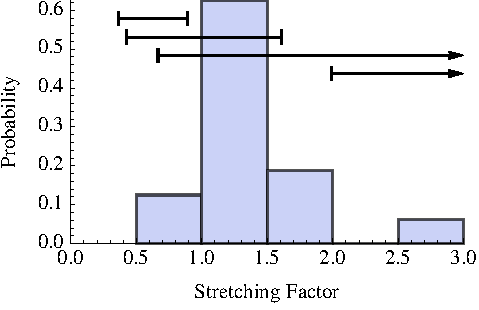
\includegraphics[width=\textwidth]{kappaDistributionHistogram}
		\label{fig:kappaDistributionHistogram}
		\caption{Histogram (blue) obtained from the model. Bar lines (black) show observed stretching factors.}
	\end{subfigure}
	\hfill
	\begin{subfigure}{0.45\textwidth}
		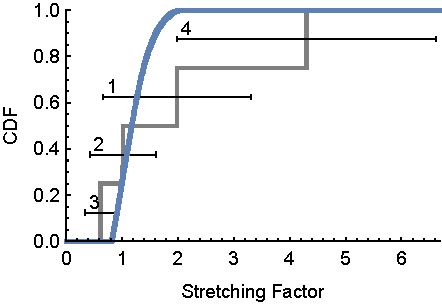
\includegraphics[width=\textwidth]{kappaDistributionCDF}
		\label{fig:kappaDistributionCDF}
		\caption{CDF (blue) obtained from the model. Gray curve and bar lines show observed stretching factors.}
	\end{subfigure}
	\hspace*{\fill}
	\caption{Stretching factors histogram and CDF produced by our model. The sample contains $4096$ bursts.}
	\label{fig:kappaDistribution}
\end{figure}

\begin{figure}
        \centering
        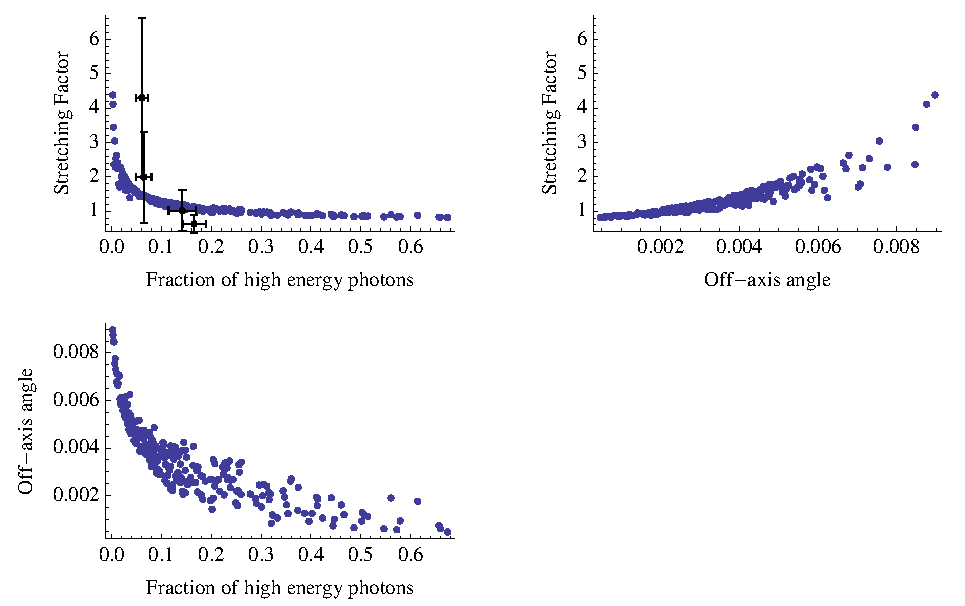
\includegraphics[width=1.0\textwidth]{correlations}
        \caption{Correlations between off-axis angles, stretching factors and high to low energy photon count ratios found in the sample produced by our model. The sample contains $4096$ bursts. Black crosses show observations with $2\sigma$ error bars. This correlation allows one to estimate off-axis angles of observed bursts.}
        \label{fig:correlations}
\end{figure}

\section{Discussion}

\label{sec:discussion}

	The main results of our study may be summarized as following:
	\begin{enumerate}
		\item{
			The time stretching of GRB light curves between different VHE bands is confirmed with statistical significance of $3.3\sigma$.
		}
		\item{
			This time stretching can be explained by geometry of the jet, without introducing any new spectral components.
		}
		\item{
			All GRBs can be assumed to be the same in their rest frames.
			There is no need to vary internal burst parameters.
		}
	\end{enumerate}

	There are, however, directions for improvement:
	\begin{itemize}
		\item{
			The model prediction and observations on fig. \ref{fig:correlations} are, though close, not exactly agree.
		}
		\item{
			Shapes of light curves produced by the model differ considerably from observed ones.
		}
		\item{
			Assumption of energy dependence on off-axis angle should be justified better.
		}
		\item{
			While we believe that all bursts are almost the same in their rest frames, they are certainly not exactly the same.
			The minor differences between GRBs might be responsible for observable deviations from the model predictions.
		}
	\end{itemize}

	We believe, however, that these problems are not unresolvable, and may be addressed by refining the model without changing its main assumptions.

	{\small {\it Acknowledgments.} The work was supported by Russian Science Foundation grant 14-12-01340.}

\bibliographystyle{hep}
\bibliography{gammaRays.bib}

\end{document}